\documentclass[journal]{vgtc}                     % final (journal style)
%\documentclass[journal,hideappendix]{vgtc}        % final (journal style) without appendices
%\documentclass[review,journal]{vgtc}              % review (journal style)
%\documentclass[review,journal,hideappendix]{vgtc} % review (journal style)
%\documentclass[widereview]{vgtc}                  % wide-spaced review
%\documentclass[preprint,journal]{vgtc}            % preprint (journal style)


%% Uncomment one of the lines above depending on where your paper is
%% in the conference process. ``review'' and ``widereview'' are for review
%% submission, ``preprint'' is for pre-publication in an open access repository,
%% and the final version doesn't use a specific qualifier.

%% If you are submitting a paper to a conference for review with a double
%% blind reviewing process, please use one of the ``review'' options and replace the value ``0'' below with your
%% OnlineID. Otherwise, you may safely leave it at ``0''.
\onlineid{0}

%% In preprint mode you may define your own headline. If not, the default IEEE copyright message will appear in preprint mode.
%\preprinttext{To appear in IEEE Transactions on Visualization and Computer Graphics.}

%% In preprint mode, this adds a link to the version of the paper on IEEEXplore
%% Uncomment this line when you produce a preprint version of the article 
%% after the article receives a DOI for the paper from IEEE
%\ieeedoi{xx.xxxx/TVCG.201x.xxxxxxx}

%% declare the category of your paper, only shown in review mode
\vgtccategory{Research}

%% please declare the paper type of your paper to help reviewers, only shown in review mode
%% choices:
%% * algorithm/technique
%% * application/design study
%% * evaluation
%% * system
%% * theory/model
\vgtcpapertype{application/design study}

%% Paper title.
\title{ExcavatorVR - Simulating an Excavator in Virtual Reality}

%% Author ORCID IDs should be specified using \authororcid like below inside
%% of the \author command. ORCID IDs can be registered at https://orcid.org/.
%% Include only the 16-digit dashed ID.
\author{%
  Sebastian Gradwohl*
}

\authorfooter{
  %% insert punctuation at end of each item
  \item
  	* Sebastian Gradwohl  is a Software Engineering Student of the University of Applied Sciences Upper Austria - Hagenberg

  	E-mail: s2310307057@fhooe.at
}

%% Abstract section.
\abstract{%
  This paper focusses on the design and implementation of a fully simulated excavator-driving environment for the Oculus Rift-S. The Goal was to simulate the controls of a real excavator as accurate as possible.
}

%% Keywords that describe your work. Will show as 'Index Terms' in journal
%% please capitalize first letter and insert punctuation after last keyword
\keywords{Virtual Reality, Machine Controls}

% A teaser figure can be included as follows
\teaser{
  \centering
  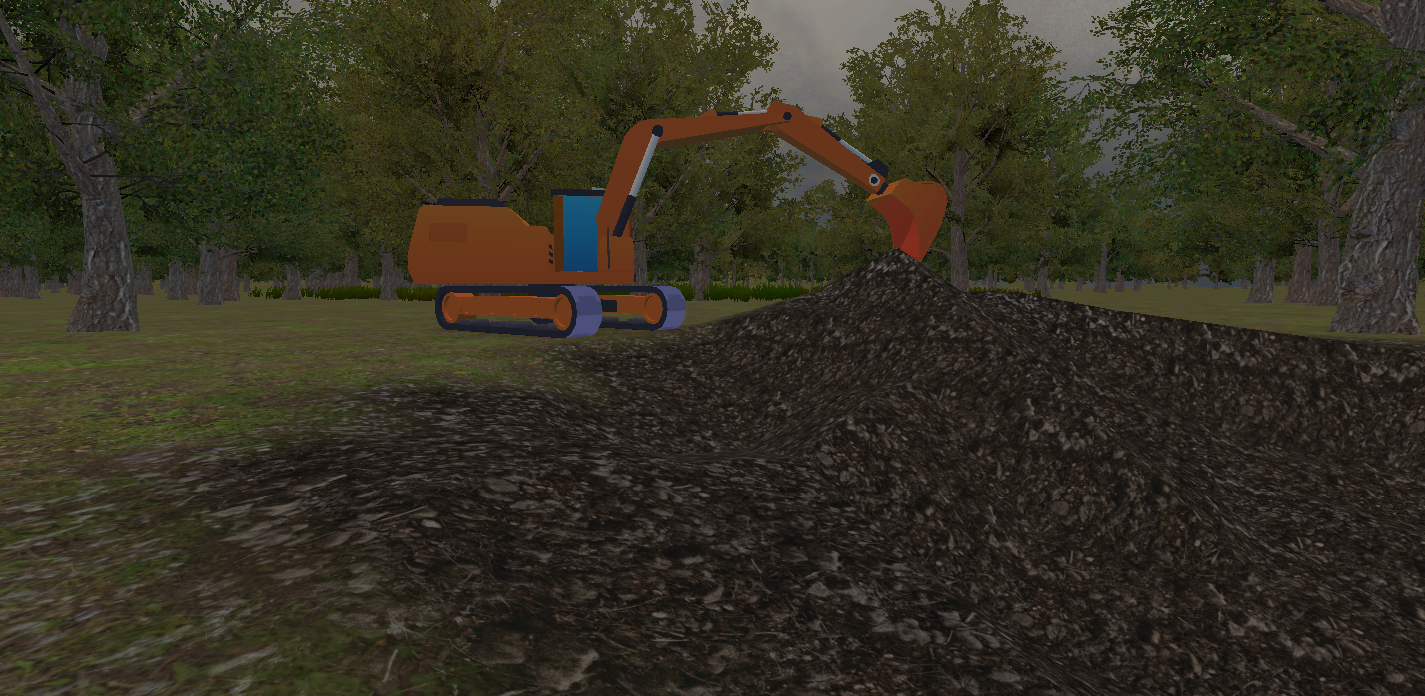
\includegraphics[width=\linewidth, alt={Outside View of the Excavator after digging out an area}]{ExcavatorOutsideView}
  \caption{%
  	An outside view from the excavator after a quick playtest to dig out a smaller area%
  }
  \label{fig:teaser}
}

%% Uncomment below to disable the manuscript note
\renewcommand{\manuscriptnotetxt}{}

%% Copyright space is enabled by default as required by guidelines.
%% It is disabled by the 'review' option or via the following command:
%\nocopyrightspace


%%%%%%%%%%%%%%%%%%%%%%%%%%%%%%%%%%%%%%%%%%%%%%%%%%%%%%%%%%%%%%%%
%%%%%%%%%%%%%%%%%%%%%% LOAD PACKAGES %%%%%%%%%%%%%%%%%%%%%%%%%%%
%%%%%%%%%%%%%%%%%%%%%%%%%%%%%%%%%%%%%%%%%%%%%%%%%%%%%%%%%%%%%%%%

%% Tell graphicx where to find files for figures when calling \includegraphics.
%% Note that due to the \DeclareGraphicsExtensions{} call it is no longer necessary
%% to provide the the path and extension of a graphics file:
%% 
\includegraphics{diamondrule} is completely sufficient.
\graphicspath{{figs/}{figures/}{pictures/}{images/}{./}} % where to search for the images

%% Only used in the template examples. You can remove these lines.
\usepackage{tabu}                      % only used for the table example
\usepackage{booktabs}                  % only used for the table example
\usepackage{lipsum}                    % used to generate placeholder text
\usepackage{mwe}                       % used to generate placeholder figures

%% We encourage the use of mathptmx for consistent usage of times font
%% throughout the proceedings. However, if you encounter conflicts
%% with other math-related packages, you may want to disable it.
\usepackage{mathptmx}                  % use matching math font

\begin{document}

%%%%%%%%%%%%%%%%%%%%%%%%%%%%%%%%%%%%%%%%%%%%%%%%%%%%%%%%%%%%%%%%
%%%%%%%%%%%%%%%%%%%%%% START OF THE PAPER %%%%%%%%%%%%%%%%%%%%%%
%%%%%%%%%%%%%%%%%%%%%%%%%%%%%%%%%%%%%%%%%%%%%%%%%%%%%%%%%%%%%%%%

%% The ``\maketitle'' command must be the first command after the
%% ``\begin{document}'' command. It prepares and prints the title block.
%% the only exception to this rule is the \firstsection command#
\firstsection{Introduction}

\maketitle


%% \section{Introduction} %for journal use above \firstsection{..} instead
Over the years there have been many attempts and demos to try and create training and demo simulators for different kinds of jobs. Virtual Reality provides an irreplacable opportunity to make the experience as realistic and easy to use as possible.
Many different industries are already creating such software and distributing it, either for their customers or for their own employees. 

Such software allows the users to train for the job in a safe space where the risk of accidents can be severely reduced whilst the economical and health dangers surrounding these are minimized.

During the conception of this project, the severe lack of training software for the construction industry in particular really stuck out. 
Therefore, in this context, the decision was made to create a small training simulator for excavator operators. Excavators have a comparatively high complexity for their controls and require a good intuition to use the machine effectively, which made this kind of vehicle the choice for this project.

\section{User Guide}

This Project is designed to be played in a seated manner. The User is not supposed to change their position during the duration of the playsession. The Chair should be placed in the middle of the playspace and should face to the front of the configured playspace of the HMDs software.

\begin{figure}[tb]% specify a combination of t, b, p, or h for top, bottom, on its own page, or here
  \centering % avoid the use of \begin{center}...\end{center} and use \centering instead (more compact)
  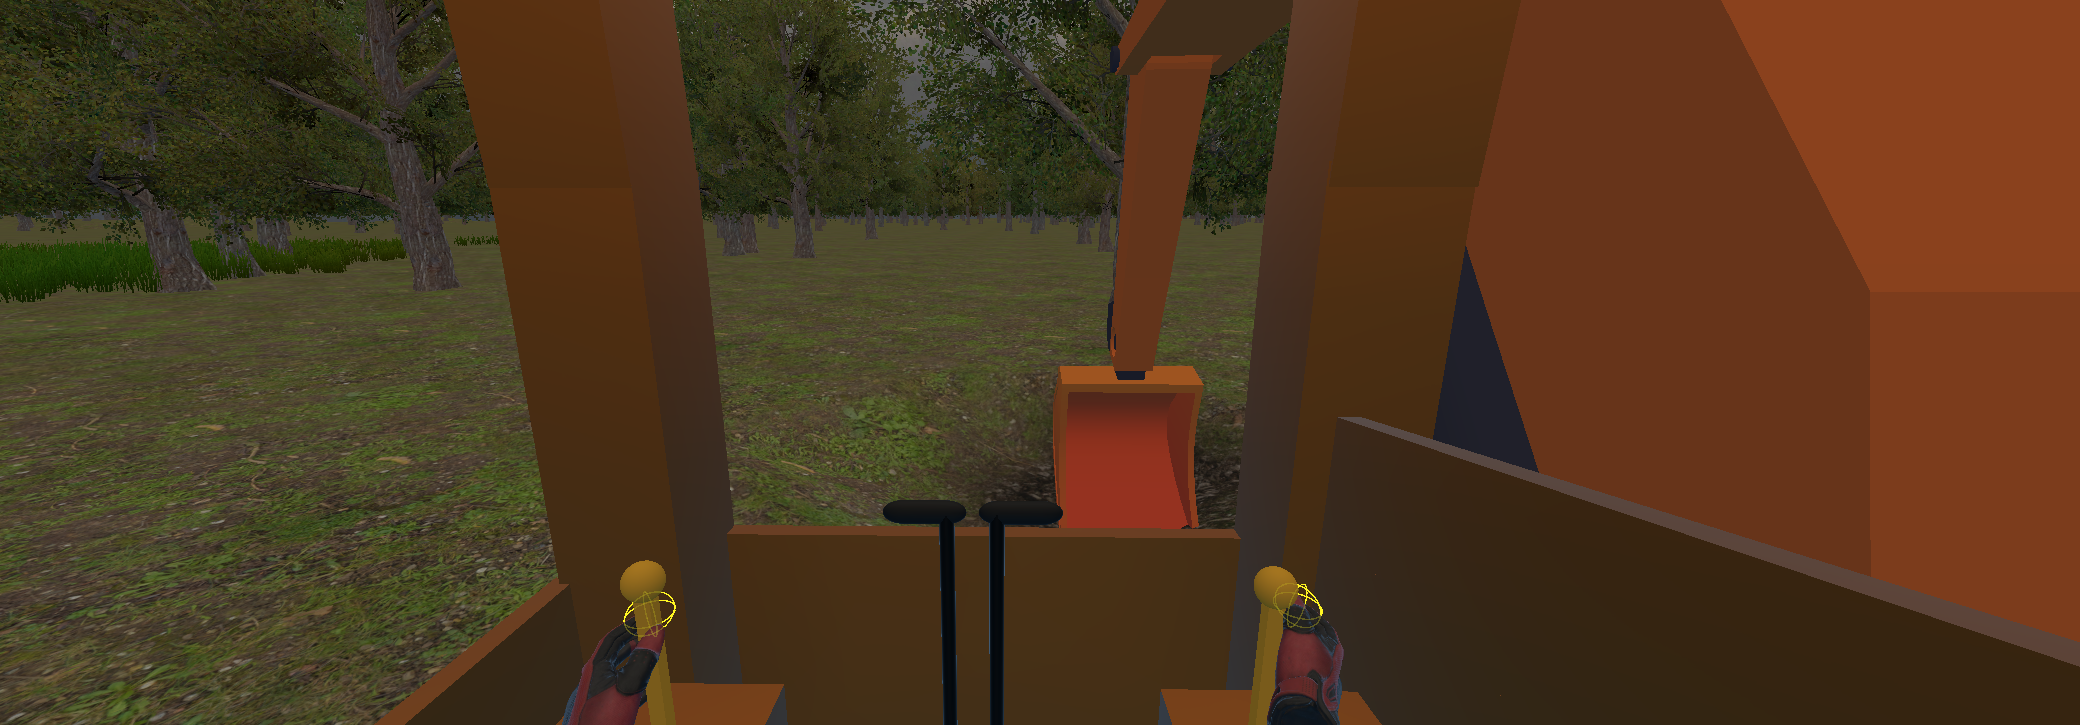
\includegraphics[width=\columnwidth, alt={The view from the cabin of a excavator. Each hand is on the joystick for controlling the vehicles arms and body}]{ExcavatorCabinView}
  \caption{%
  	The View of the player during his VR experience%
  }
  \label{fig:cabin_view}
\end{figure}

\subsection{First Steps}
After Startup the User is immediately placed into the drivers seat of their excavator. On the left and right console there is a grabbable joystick each and in front of the seat there are two levers. 

The Controls of the excavator are based on the ISO Standard 10968. This Standard defines the following controls for the excavator:

\begin{itemize}
  \item The left joystick tilting left causes the excavators upper body to swing left
  \item The left joystick tilting right causes the excavators upper body to swing right
  \item The left joystick tilting forward causes the excavators dipper, also known as stick boom, to move away.
           The Stick Boom of the excavator is the second half of the excavators arm, connecting the main boom with the bucket.
  \item The left joystick tilting backwards causes the excavators stick boom, to move closer.
  \item The right joystick tilting left causes the bucket of the excavator to curl in, therefore closing
  \item The right joystick tilting right causes the bucket of the excavator to curl out. Thereby allowing for the bucket to dump its contents
  \item The right joystick tilting forward causes the main boom and therefore the entire arm to go down
  \item The right joystick tilting backwards causes the main boom to go back up 
  \item The left lever in front of the seat defines the movement of the left track of the excavator. The further it gets tilted, the faster the track moves. If it gets tilted backwards, the track moves backwards instead.
  \item The right lever in front of the seat defines the movement of the right track of the excavator. The further it gets tilted, the faster the track moves. If it gets tilted backwards, the track moves backwards instead.
\end{itemize}

Theoretically there is a second standard for the controls, SAE J1814, inverting the main and stick booms controls compared to ISO 10968, but for now the focus was put on the ISO standard.

The interaction is possible by hovering over the object to be controlled with a hand and then pressing the controllers grip button. For the Track-Levers the forward or Backward movement of the hand is translated into the lever moving forward or backwards. For the Joysticks a different methodology had to be found, due to the translation of 360° Movement into a translatable rotation proved more difficult than first expected. Therefore the behavior for the joysticks was made to relay the rotation movement of the hand to the joystick. Thanks for the joysticks being rather small this solution works quite well. The smaller size of the Joystick would make moving ones hand further away and still controlling the joystick rather unrealistic and unintuitive in comparison to the larger Track-Levers.

\section{Design}

While a VR Project comes with alot of weaknesses inherent to the nature of the current hardware, it also provides alot of possibilities and strengths which are impossible to reproduce with other forms of media.
The goal of this project was to use as many of the strengths whilst avoiding or mitigating the many pitfalls alot of VR software is commonly affected by, such as motion sickness or high latency with the interactions


\subsection{Keeping it simple}

Freedom often leads to confusion. Therefore the goal was to streamline the user experience in a way, where the user is not overwhelmed and neither completely left to their own devices. This is managed through a few smaller systems and design decisions


\subsection{Seated like in reality}

Due to the focus being on simulating an excavator operators experience the decision was made to keep the user in the same location at all times. Whilst movement is still allowed, to enable the user to for example look out of the window of the vehicle, there is no incentive to leave the seated area.

This decision also avoids alot of issues concerning motion sickness. Due to the user being in a seated position and the velocity of the excavator being rather slow by nature, moving with the excavator is not nausea inducing and should therefore make the simulation alot more accessible to users with less to no experience with Virtual Reality.


\begin{figure}[tb]% specify a combination of t, b, p, or h for top, bottom, on its own page, or here
  \centering % avoid the use of \begin{center}...\end{center} and use \centering instead (more compact)
  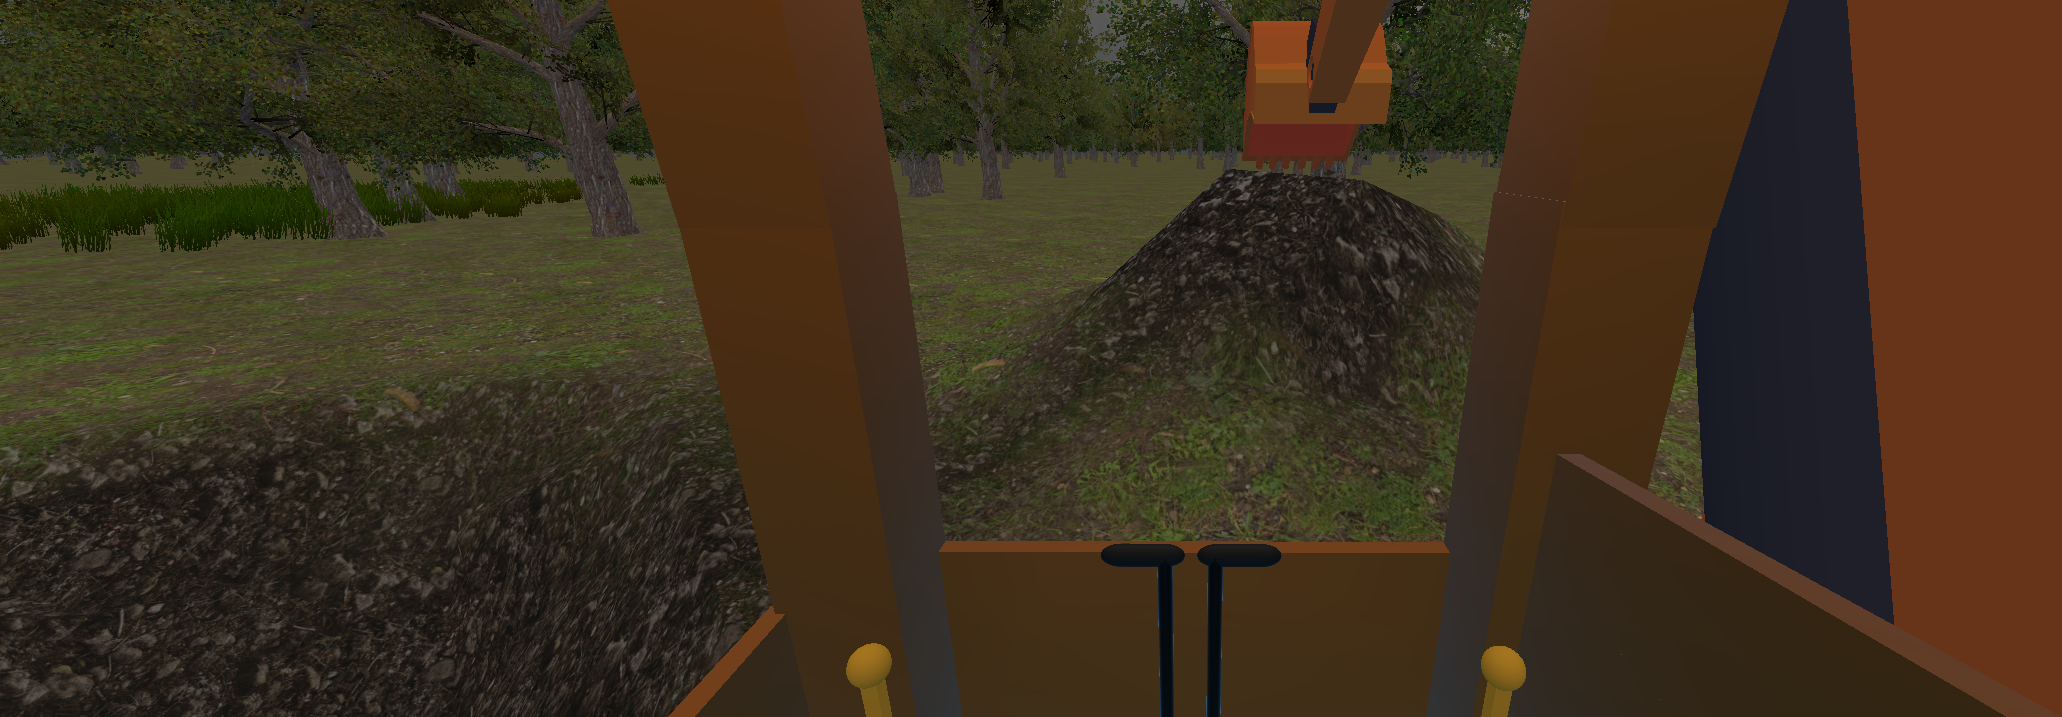
\includegraphics[width=\columnwidth, alt={The view from the cabin of a excavator. On one side there is a smaller hole, next to it lies a small heap of material, suggesting the excavator dug it out. the shovel is placed neatly on top of the heap}]{GroundDeformation}
  \caption{%
  	The View from the cabin after excavating a small hole and dumping material to create a small heap%
  }
  \label{fig:cabin_view}
\end{figure}

\subsection{The world confirms the excavators existance}

One important aspect the simulation was of course the excavator buckets behavior. After all, getting a hang of the controls to move each component of an excavator effectively is only the beginning. Therefore it was essential to implement the most common task of excavators: The movement of material through an area by digging it away and dumping it somewhere else.

Therefore it was important to make the shovel interact with the surrounding terrain of the excavator, allowing for it to create holes when digging and to dump material when opening the shovel over the terrain.


\section{Implementation}



\subsection{}

The style automatically looks for image files with the correct extension (eps for regular \LaTeX; pdf, png, and jpg for pdf\LaTeX), in a set of given subfolders defined above using \verb|\graphicspath|: figures/, pictures/, images/.
It is thus sufficient to use \verb|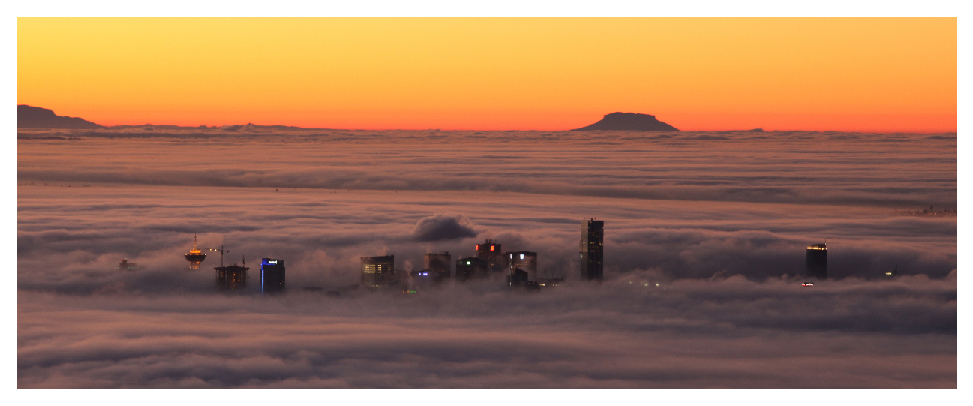
\includegraphics{CypressView}| (instead of \verb|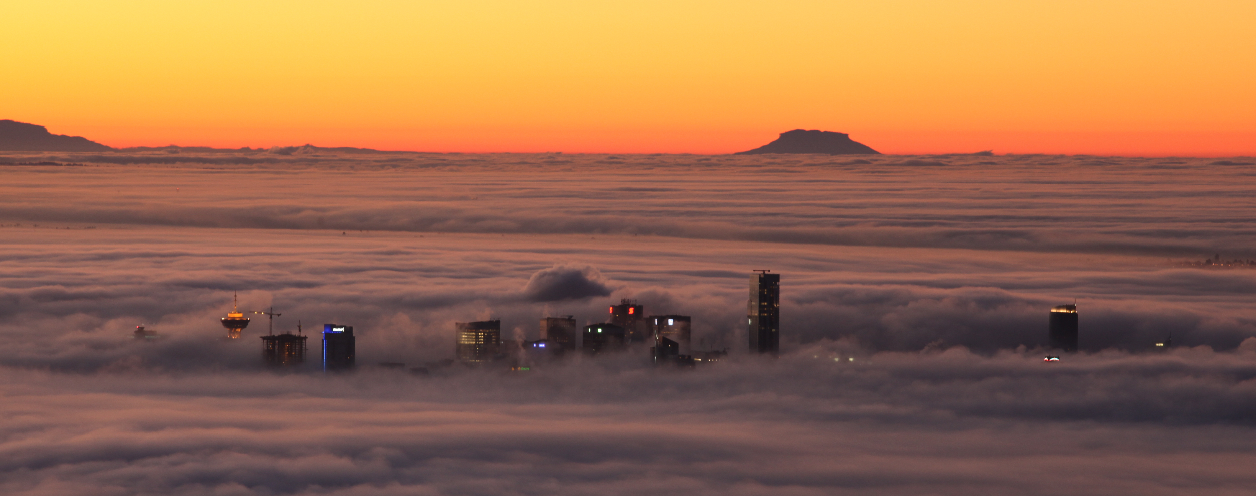
\includegraphics{pictures/CypressView.jpg}|).
Figures should be in CMYK or Grey scale format, otherwise, colour shifting may occur during the printing process.

\subsection{Vector figures}

Vector graphics like svg, eps, pdf are best for charts and other figures with text or lines.
They will look much nicer and crisper and any text in them will be more selectable, searchable, and accessible.

\subsection{Raster figures}

Of the raster graphics formats, screenshots of user interfaces and text, as well as line art, are better shown with png.
jpg is better for photographs.
Make sure all raster graphics are captured in high enough resolution so they look crisp and scale well.

\subsection{Alt texts}

Add alternative texts that describe the content of the image to all figures.

\subsection{Figures on the first page}

The teaser figure should only have the width of the abstract as the template enforces it.
The use of figures other than the optional teaser is not permitted on the first page.
Other figures should begin on the second page.
Papers submitted with figures other than the optional teaser on the first page will be refused.

\subsection{Subfigures}

\subsection{Figure Credits}
\label{sec:figure_credits_inst}

In the \hyperref[sec:figure_credits]{Figure Credits} section at the end of the paper, you should credit the original sources of any figures that were reproduced or modified.
Include any license details necessary, as well as links to the original materials whenever possible.
For credits to figures from academic papers, include a citation that is listed in the \textbf{References} section.
An example is provided \hyperref[sec:figure_credits]{below}.


\section{Equations and Tables}

Equations can be added like so:

\begin{equation}
  \label{eq:sum}
  \sum_{j=1}^{z} j = \frac{z(z+1)}{2}
\end{equation}

Tables, such as \cref{tab:vis_papers} can also be included.


\begin{table}[tb]
  \caption{%
  	VIS/VisWeek accepted/presented papers: 1990--2016.%
  }
  \label{tab:vis_papers}
  \scriptsize%
  \centering%
  \begin{tabu}{%
  	  r%
  	  	*{7}{c}%
  	  	*{2}{r}%
  	}
  	\toprule
  	year & \rotatebox{90}{Vis/SciVis} &   \rotatebox{90}{SciVis conf} &   \rotatebox{90}{InfoVis} &   \rotatebox{90}{VAST} &   \rotatebox{90}{VAST conf} &   \rotatebox{90}{TVCG @ VIS} &   \rotatebox{90}{CG\&A @ VIS} &   \rotatebox{90}{VIS/VisWeek} \rotatebox{90}{incl.\ TVCG/CG\&A}   &   \rotatebox{90}{VIS/VisWeek} \rotatebox{90}{w/o TVCG/CG\&A}   \\
  	\midrule
  	2016 & 30 &   & 37 & 33 & 15 & 23 & 10 & 148 & 115 \\
  	2015 & 33 & 9 & 38 & 33 & 14 & 17 & 15 & 159 & 127 \\
  	2014 & 34 &   & 45 & 33 & 21 & 20 &    & 153 & 133 \\
  	2013 & 31 &   & 38 & 32 &    & 20 &    & 121 & 101 \\
  	2012 & 42 &   & 44 & 30 &    & 23 &    & 139 & 116 \\
  	2011 & 49 &   & 44 & 26 &    & 20 &    & 139 & 119 \\
  	2010 & 48 &   & 35 & 26 &    &    &    & 109 & 109 \\
  	2009 & 54 &   & 37 & 26 &    &    &    & 117 & 117 \\
  	2008 & 50 &   & 28 & 21 &    &    &    &  99 &  99 \\
  	2007 & 56 &   & 27 & 24 &    &    &    & 107 & 107 \\
  	2006 & 63 &   & 24 & 26 &    &    &    & 113 & 113 \\
  	2005 & 88 &   & 31 &    &    &    &    & 119 & 119 \\
  	2004 & 70 &   & 27 &    &    &    &    &  97 &  97 \\
  	2003 & 74 &   & 29 &    &    &    &    & 103 & 103 \\
  	2002 & 78 &   & 23 &    &    &    &    & 101 & 101 \\
  	2001 & 74 &   & 22 &    &    &    &    &  96 &  96 \\
  	2000 & 73 &   & 20 &    &    &    &    &  93 &  93 \\
  	1999 & 69 &   & 19 &    &    &    &    &  88 &  88 \\
  	1998 & 72 &   & 18 &    &    &    &    &  90 &  90 \\
  	1997 & 72 &   & 16 &    &    &    &    &  88 &  88 \\
  	1996 & 65 &   & 12 &    &    &    &    &  77 &  77 \\
  	1995 & 56 &   & 18 &    &    &    &    &  74 &  74 \\
  	1994 & 53 &   &    &    &    &    &    &  53 &  53 \\
  	1993 & 55 &   &    &    &    &    &    &  55 &  55 \\
  	1992 & 53 &   &    &    &    &    &    &  53 &  53 \\
  	1991 & 50 &   &    &    &    &    &    &  50 &  50 \\
  	1990 & 53 &   &    &    &    &    &    &  53 &  53 \\
  	\midrule               
  	\textbf{sum} & \textbf{1545} & \textbf{9} & \textbf{632} & \textbf{310} & \textbf{50} & \textbf{123} & \textbf{25} & \textbf{2694} & \textbf{2546} \\
  	\bottomrule
  \end{tabu}%
\end{table}

\section{Supplemental Material Instructions}
\label{sec:supplement_inst}

In support of transparent research practices and long-term open science goals, you are encouraged to make your supplemental materials available on a publicly-accessible repository.
Please describe the available supplemental materials in the \hyperref[sec:supplemental_materials]{Supplemental Materials} section.
These details could include (1) what materials are available, (2) where they are hosted, and (3) any necessary omissions.


\section{References}
\label{sec:references_inst}

An example of the reference formatting is provided in the \textbf{References} section at the end.


\subsection{Include DOIs}

All references which have a DOI should have it included in the bib\TeX\ for the style to display.
The DOI can be entered with or without the \url{https://doi.org/} prefix.

\subsection{Narrow DOI option}

The \verb|-narrow| versions of the bibliography style use the font \verb|PTSansNarrow-TLF| for typesetting the DOIs in a compact way.
This font needs to be available on your \LaTeX\ system.
It is part of the \href{https://www.ctan.org/pkg/paratype}{\texttt{paratype} package}, and many distributions (such as MikTeX) have it automatically installed.
If you do not have this package yet and want to use a \verb|-narrow| bibliography style then use your \LaTeX\ system's package installer to add it.
If this is not possible you can also revert to the respective bibliography styles without the \verb|-narrow| in the file name.
DVI-based processes to compile the template apparently cannot handle the different font so, by default, the template file uses the \texttt{abbrv-doi} bibliography style.

\subsection{Disabling hyperlinks}

To avoid adding hyperlinks to the references (the default) you can use \verb|\bibliographystyle{abbrv-doi}| instead of \verb|\bibliographystyle{abbrv-doi-hyperref}|.
By default, the DOI field in a bib\TeX\ entry is turned into a hyperlink.

See the examples in the bib\TeX\ file and the bibliography at the end of this template.

\subsection{Guidelines for bibTeX}

\begin{itemize}
  \item All bibliographic entries should be sorted alphabetically by the last name of the first author.
        This \LaTeX/bib\TeX\ template takes care of this sorting automatically.
  \item Merge multiple references into one; e.\,g., use \cite{Max1995OpticalModelsDirect,Kitware2003VisualizationToolkitUsers} (not \cite{Kitware2003VisualizationToolkitUsers}\cite{Max1995OpticalModelsDirect}).
        Within each set of multiple references, the references should be sorted in ascending order.
        This \LaTeX/bib\TeX\ template takes care of both the merging and the sorting automatically.
  \item Verify all data obtained from digital libraries, even ACM's DL and IEEE Xplore  etc.\ are sometimes wrong or incomplete.
  \item Do not trust bibliographic data from other services such as Mendeley.com, Google Scholar, or similar; these are even more likely to be incorrect or incomplete.
  \item Articles in journal---items to include:
        \begin{itemize}
  	      \item author names
  	      \item title
  	      \item journal name
  	      \item year
  	      \item volume
  	      \item number
  	      \item month of publication as variable name (i.e., \{jan\} for January, etc.; month ranges using \{jan \#\{/\}\# feb\} or \{jan \#\{-{}-\}\# feb\})
          \item series. E.g., ``TVCG``, ``TVCG/VIS`` for special issue VIS papers, ``EuroVis``, ``CGF/EuroVis``.
        \end{itemize}
  \item Use journal names in proper style: correct: ``IEEE Transactions on Visualization and Computer Graphics'', incorrect: ``Visualization and Computer Graphics, IEEE Transactions on''
  \item Papers in proceedings---items to include:
        \begin{itemize}
  	      \item author names
  	      \item title
  	      \item abbreviated proceedings name: e.g., ``Proc.\textbackslash{} CONF\_ACRONYNM'' without the year; example: ``Proc.\textbackslash{} CHI'', ``Proc.\textbackslash{} 3DUI'', ``Proc.\textbackslash{} Eurographics'', ``Proc.\textbackslash{} EuroVis''
  	      \item year
  	      \item series. E.g., ``VIS`` and ``EuroVis`` for short papers, ``CHI``...
        \end{itemize}

  \item Article/paper title convention: refrain from using curly brackets, except for acronyms/proper names/words following dashes/question marks etc.; example:\\\\
        %
        The paper ``Marching Cubes: A High Resolution 3D Surface Construction Algorithm'' should be entered as ``\{M\}arching \{C\}ubes: A High Resolution \{3D\} Surface Construction Algorithm'' or  ``\{M\}arching \{C\}ubes: A high resolution \{3D\} surface construction algorithm''.
        It will then be typeset as ``Marching Cubes: A high resolution 3D surface construction algorithm''.
  \item For all entries:
        \begin{itemize}
  	      \item DOI can be entered in the DOI field as plain DOI number or as DOI url.
  	      \item ``pages`` or ``articleno``: Provide full page ranges AA-{}-BB, OR, if an article number is available like recent ACM conferences, use that instead. E.g., see the entry for Panavas et al.\ \cite{Panavas2022JuvenileGraphicalPerception}.
        \end{itemize}
  \item When citing references, do not use the reference as a sentence object; e.g., wrong: ``In \cite{Lorensen1987MarchingCubesHigh} the authors describe \dots'', correct: ``Lorensen and Cline \cite{Lorensen1987MarchingCubesHigh} describe \dots''
\end{itemize}

\section{Appendices}
\label{sec:appendices_inst}

Appendices can be specified using \verb|\appendix|.
For example, our Troubleshooting instructions in
\iflabelexists{appendix:troubleshooting}
  {\cref{appendix:troubleshooting}}
  {the appendix of the full paper at \url{https://osf.io/nrmyc}}.

Note that the paper submission has to end after the \textbf{References} section and within the page limit of the conference you are submitting to.
Any version of Appendices or the paper with Appendices included has to be submitted separately as supplementary material.
You can use the \verb|hideappendix| class option to remove everything after \verb|\appendix|.
We encourage you to submit a full version of your paper to a preprint server with any appendices included.

You can use the \verb|\iflabelexists| macro to cross reference an appendix from the main text, but only if that label (i.e.\ the appendix) actually exists.
For example, above we use 

\begin{verbatim}
\iflabelexists{appendix:troubleshooting}
  {\cref{appendix:troubleshooting}}
  {the appendix of the full paper at
   \url{https://osf.io/XXXXX}}.
\end{verbatim}

in order to cross-reference to the appendix with \verb|\cref| if it exists, but if the appendix is commented out then we will simply create a hyperlinked URL to it.


\section{Filler Text to Flush Out the Paper}

\lipsum[1-2]% Just add some more arbitrary text so we see a fuller paper example


\section*{Supplemental Materials}
\label{sec:supplemental_materials}

Refer to the instructions for this section (\cref{sec:supplement_inst}).
Below is an example you can follow that includes the actual supplemental material for this template:

All supplemental materials are available on OSF at \url{https://doi.org/10.17605/OSF.IO/2NBSG}, released under a CC BY 4.0 license.
In particular, they include (1) Excel files containing the data for and analyses for creating \cref{tab:vis_papers} and \cref{fig:vis_papers}, (2) figure images in multiple formats, and (3) a full version of this paper with all appendices.
Our other code is intellectual property of a corporation---Starbucks Research---and there is no feasible way to share it publicly.


\section*{Figure Credits}
\label{sec:figure_credits}

Refer to the instructions for this section (\cref{sec:figure_credits_inst}).
Here are the actual figure credits for this template:

\Cref{fig:teaser} image credit: Scott Miller / Special to the Vancouver Sun, January 22, 2009, page A6.

\Cref{fig:vis_papers} is a partial recreation of Fig.\ 1 from \cite{Isenberg2017Vispubdata.orgMetadataCollection}, which is in the public domain.


%% if specified like this the section will be omitted in review mode
\acknowledgments{%
	The authors wish to thank A, B, and C.
  This work was supported in part by a grant from XYZ (\# 12345-67890).%
}


\bibliographystyle{abbrv-doi-hyperref}
%\bibliographystyle{abbrv-doi-hyperref-narrow}
%\bibliographystyle{abbrv-doi}
%\bibliographystyle{abbrv-doi-narrow}

\bibliography{template}


\appendix % You can use the `hideappendix` class option to skip everything after \appendix

\section{About Appendices}
Refer to \cref{sec:appendices_inst} for instructions regarding appendices.

\section{Troubleshooting}
\label{appendix:troubleshooting}

\subsection{ifpdf error}

If you receive compilation errors along the lines of \texttt{Package ifpdf Error: Name clash, \textbackslash ifpdf is already defined} then please add a new line \verb|\let\ifpdf\relax| right after the \verb|\documentclass[journal]{vgtc}| call.
Note that your error is due to packages you use that define \verb|\ifpdf| which is obsolete (the result is that \verb|\ifpdf| is defined twice); these packages should be changed to use \verb|ifpdf| package instead.


\subsection{\texttt{pdfendlink} error}

Occasionally (for some \LaTeX\ distributions) this hyper-linked bib\TeX\ style may lead to \textbf{compilation errors} (\texttt{pdfendlink ended up in different nesting level ...}) if a reference entry is broken across two pages (due to a bug in \verb|hyperref|).
In this case, make sure you have the latest version of the \verb|hyperref| package (i.e.\ update your \LaTeX\ installation/packages) or, alternatively, revert back to \verb|\bibliographystyle{abbrv-doi}| (at the expense of removing hyperlinks from the bibliography) and try \verb|\bibliographystyle{abbrv-doi-hyperref}| again after some more editing.

\end{document}

